% Rendered with xelatex. NeurIPS-style theme; Korean via kotex (AppleMyungjo) + Times.
\documentclass[10pt]{article}
\usepackage[letterpaper,left=1.1in,right=1.1in,top=0.8in,bottom=0.8in]{geometry}
\usepackage{kotex}
\usepackage{fontspec}
\setmainfont{Times New Roman}
\setmainhangulfont{AppleMyungjo}[AutoFakeBold=2.2]
\usepackage{amsmath,amssymb}
\usepackage{graphicx}
\usepackage{booktabs}
\usepackage{float}
\usepackage[font=small,labelfont=bf,skip=4pt]{caption}
\usepackage{subcaption}
\usepackage{titlesec}
\titleformat{\section}{\large\bfseries}{\thesection}{0.6em}{}
\titlespacing*{\section}{0pt}{6pt}{2pt}
\setlength{\parskip}{1pt}
\usepackage[colorlinks=true,allcolors=blue]{hyperref}

\newcommand{\abc}{$\alpha,\beta$-CROWN}
\newcommand{\linf}{$\ell_\infty$}
\newcommand{\eps}{$\varepsilon$}

\begin{document}

\begin{center}
  {\LARGE\bfseries MNIST 분류기의 Bound-Propagation 강건성 검증:\\[2pt]
   $\alpha,\beta$-CROWN과 Marabou 비교}\\[10pt]
  {\normalsize 백재민}\\[2pt]
  \rule{\textwidth}{0.4pt}
\end{center}

\begin{center}\textbf{초록}\end{center}
\begin{quote}\small
소형 완전연결 MNIST 분류기의 국소 \linf{} 강건성을 \abc{}로 검증하고, 동일한 인스턴스에서
이전에 사용한 SMT 기반 검증기 Marabou와 비교한다. 두 도구는 공유된 모든 판정과 샘플별
강건성 임계값에서 일치했으며, 이를 건전성(soundness) 교차검증으로 활용한다. 흥미로운 차이는
정량적이다: 속도 격차는 상수가 아니라 특정 \eps{}에서 벌어지고, 검증 노력은 좁은 \eps{}
구간에서 값싼 bound로부터 branch-and-bound로 옮겨가며, 모든 반례는 탐색이 아니라 공격으로
발견되고, 어려운 인스턴스의 성패는 솔버가 아니라 분기 휴리스틱 선택이 좌우한다.
\end{quote}

\section{설정}
\textbf{모델과 데이터.} 네트워크는 ReLU 활성(은닉 96개)을 갖는 완전연결 분류기
$784\!\to\!64\!\to\!32\!\to\!10$이며, ONNX로 내보내 Marabou 연구에서 그대로 재사용했다.
두 도구가 \emph{동일한} 네트워크를 \emph{동일한} 입력에서 검증하도록 하기 위함이다. 입력은
MNIST 테스트 이미지로, 평균 $0.1307$, 표준편차 $0.3081$로 정규화되어 값이
$[-0.4242, 2.8215]$에 놓인다.

\textbf{속성.} 입력 $x$(정답 $L$)와 반경 \eps{}에 대해 국소 \linf{} 강건성을 검증한다:
$\lVert x'-x\rVert_\infty \le \varepsilon$(유효 범위로 clip)인 모든 $x'$에서 네트워크가 $L$을
arg-max로 유지하는가. Marabou 질의와 정확히 맞추기 위해 섭동을 \emph{정규화 공간}에 적용한
per-instance VNNLIB로 인코딩한다(UNSAT $\Rightarrow$ 검증됨, SAT $\Rightarrow$ 반증됨). \abc{}는
CPU에서 branch-and-bound(Gurobi 미사용), \texttt{kfsb} 분기 휴리스틱으로 실행한다.

\section{결과 및 해석}
\textbf{Phase 1 --- 스캔 (100샘플, $\varepsilon=0.05$).} 96개 강건 검증, 4개 반증
(샘플 8, 33, 92, 96), timeout 0; 인스턴스당 평균 $0.21$\,초.

\textbf{Phase 2 --- 임계값.} 반증되는 최소 \eps{}는 샘플 8이 $0.03$, 샘플 33이 $0.05$이며,
샘플 0은 $\varepsilon=0.20$까지 강건하다. 이는 Marabou 임계값과 정확히 일치한다.

\textbf{속도 우위는 상수가 아니라 \eps{}에 의존한다.} 강건 샘플 0에서 작은 반경일 때 두 도구는
사실상 동률이고($\varepsilon=0.01$: Marabou $0.39$\,초, \abc{} $0.30$\,초), $\varepsilon=0.11$까지
비등하다(Marabou $1.0$\,초). 이후 Marabou는 급격히 악화되어 $\varepsilon=0.12$에서 $6.2$\,초,
$\varepsilon\ge0.19$에서 $300$\,초 timeout에 이르는 반면, \abc{}는 $\varepsilon=0.20$에서도
$1.5$\,초에 그친다(그림~\ref{fig:plots}a). 흔히 인용되는 ${\sim}270\times$ 격차는 \emph{꼬리}의
성질이며, 정직한 요약은 ``$\varepsilon\approx0.11$까지 대등, 이후 SMT 탐색이 급락''이다.

\textbf{노력이 어디로 가는가, 그리고 급격한 전이.} 100개 인스턴스가 각각 어떻게 해결되는지를
분해하면(그림~\ref{fig:plots}b), 값싼 incomplete CROWN bound가 $\varepsilon\le0.02$에서는 100개
모두를, 그러나 $\varepsilon=0.20$에서는 단 5개만 해결한다. branch-and-bound 비중은
$\varepsilon\approx0.12$--$0.15$의 좁은 구간에서 가파르게 상승한다. 검증 난이도는 \eps{} 전반에
고르게 퍼진 것이 아니라 한 구간에 집중되어 있다.

\textbf{모든 반례는 탐색이 아니라 공격에서 나온다.} 모든 \eps{}에서 반증 인스턴스는 PGD
공격(\texttt{unsafe-pgd})으로 해결되며 branch-and-bound로는 결코 해결되지 않는다
(\texttt{unsafe-bab} $=0$). 이 네트워크에서는 값싼 공격만으로도 반증이 충분하며, 비싼 완전
탐색은 거의 전적으로 강건성을 \emph{증명}하는 데 쓰인다. 복원된 반례는 뚜렷한 오분류이다
(예: 샘플 8: $5\!\to\!6$; 33: $4\!\to\!0$; 92: $9\!\to\!4$; 96: $1\!\to\!9$), 각각 \eps{}-공
안의 작은 섭동이다(그림~\ref{fig:cex}).

\begin{figure}[H]
  \centering
  \begin{subfigure}{0.49\textwidth}\centering
    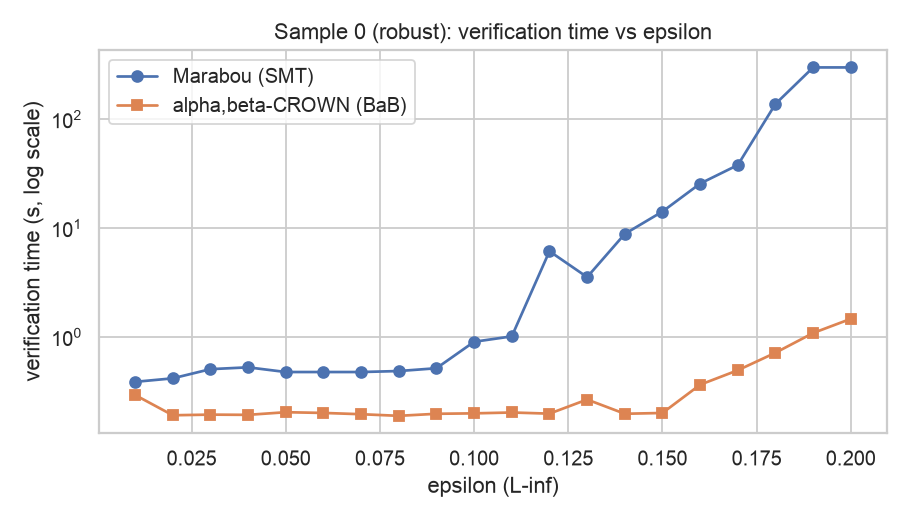
\includegraphics[width=\textwidth]{results/fig_runtime_vs_eps.png}
    \caption{}\label{fig:runtime}
  \end{subfigure}\hfill
  \begin{subfigure}{0.49\textwidth}\centering
    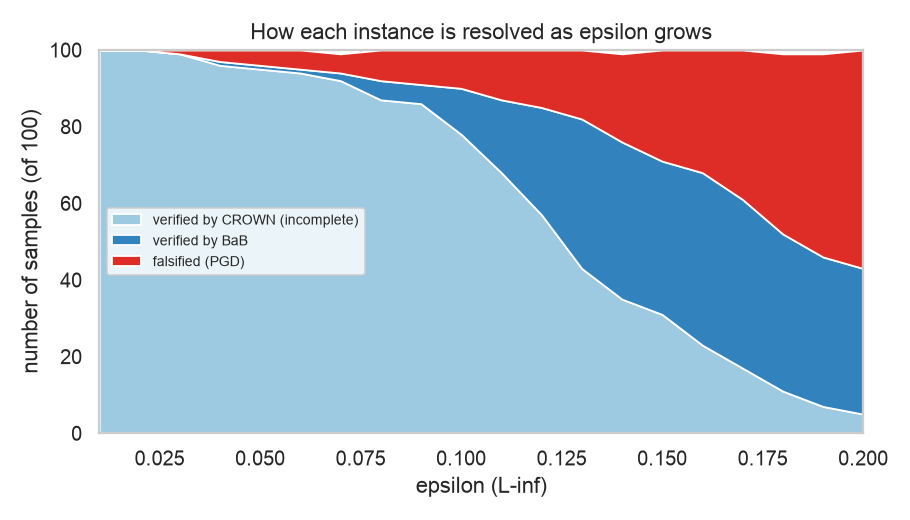
\includegraphics[width=\textwidth]{results/fig_breakdown_area.png}
    \caption{}\label{fig:breakdown}
  \end{subfigure}
  \caption{(a) 강건 샘플 0의 \eps{} 대비 검증 시간(로그 축): $\varepsilon\approx0.11$까지 비등,
  이후 Marabou는 timeout, \abc{}는 약 $1.5$\,초 유지. (b) \eps{} 증가에 따른 100개 인스턴스의
  해결 방식; branch-and-bound 비중이 $\varepsilon\approx0.12$--$0.15$에서 급증.}
  \label{fig:plots}
\end{figure}

\begin{figure}[H]
  \centering
  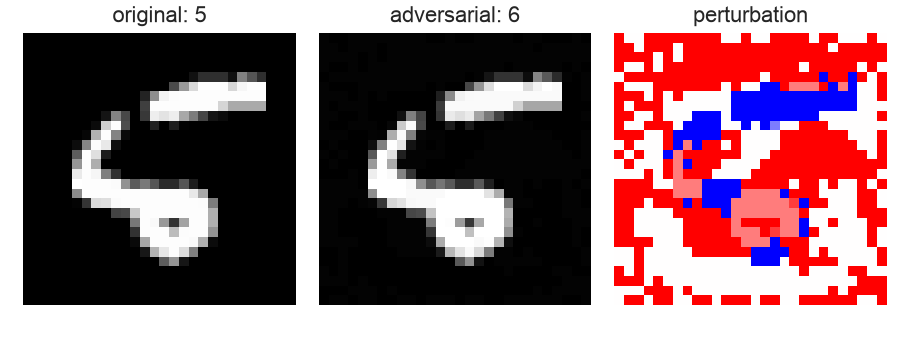
\includegraphics[width=0.46\textwidth]{results/cex_s8.png}
  \caption{$\varepsilon=0.05$에서 샘플 8의 반례(원본 $\mid$ 적대적 $\mid$ 섭동): \linf{} 섭동이
  예측을 $5\!\to\!6$으로 뒤집는다.}
  \label{fig:cex}
\end{figure}

\section{Marabou와의 비교}
\begin{table}[H]
  \centering\small
  \begin{tabular}{lll}
    \toprule
     & \abc{} & Marabou \\
    \midrule
    방법 & 선형 완화 + branch-and-bound & SMT (Reluplex) \\
    인터페이스 & 선언형 YAML + VNNLIB & 명령형 Python API \\
    공유 인스턴스 판정 & 동일 & 동일 \\
    강건 샘플, $\varepsilon=0.20$ & ${\sim}1.5$\,초 & $300$\,초 (timeout) \\
    단일 소형 쿼리(콜드 스타트) & ${\sim}2.5$\,초 & ${\sim}0.5$\,초 \\
    \bottomrule
  \end{tabular}
\end{table}

표 이외에 실험에서 얻은 세 가지를 짚는다. 첫째, \emph{일치} 자체가 결과다: 도구 간 속성을
맞추려면 VNNLIB 안에서 \eps{}를 정규화 공간에 적용해야 했고, 동일한 임계값($0.03$, $0.05$)은
인코딩이 정확함과 두 독립 엔진이 상호 일관됨을 모두 확인해 준다. 둘째, ``사용 편의성''은 양면적
이었다: \abc{}의 config 기반 배치 모드는 100샘플 스윕을 한 번의 실행으로 만들었지만, 동작하는
환경에 이르기까지 도구 특유의 마찰(Gurobi를 쓰지 않아도 강제되는 \texttt{gurobipy} import,
CPU 전용 빌드)을 처리해야 했다. 반면 Marabou의 Python API는 일회성 쿼리에 더 직접적이다.
셋째, 복원된 \emph{반례는 일치할 필요가 없다}: Marabou의 비엄격 위반 인코딩
($\text{output}[j]\ge\text{output}[L]$)은 arg-max가 정답과 동점인 점을 반환할 수 있는 반면,
\abc{}의 PGD는 엄격한 오분류를 반환한다 --- 둘 다 동일한 비강건성의 유효한 증거다.

\section{강점과 한계}
\textbf{강점.} \abc{}는 SMT가 하지 못하는 방식으로 우아하게 확장된다: 100개 테스트 샘플 전부를
값싸게 인증했고(따라서 강건성 반경 분포 전체를 도출 --- 43/100이 $\varepsilon=0.20$을 넘어서도
강건), Marabou를 timeout으로 몰아넣은 큰 \eps{}의 강건 사례들을 해결했다.

\textbf{관찰된 한계.} (i) 항상 빠른 것은 \emph{아니다}: 단일 소형 쿼리는 콜드 스타트 시
${\sim}2.5$\,초로 Marabou의 ${\sim}0.5$\,초보다 느린데, 소형 모델에서는 프로세스 시작 비용이
지배하기 때문이다. 이점은 시작 비용이 배치 전반에 amortize될 때 비로소 나타난다. (ii) 성패가
솔버가 아니라 분기 휴리스틱에 달릴 수 있다: 가장 어려운 인스턴스(샘플 22, $\varepsilon=0.2$)에서
\texttt{kfsb}는 $31$\,초에 검증했으나 \texttt{fsb}는 timeout, \texttt{babsr}는 upstream
\texttt{AttributeError}로 크래시했다. 기본값 \texttt{kfsb}는 동작했지만, 설정 표면이 넓고 균일
하게 견고하지는 않음을 보여준다.

\end{document}
